% =====================================================================
%  diagramas.tex
%  Los cuatro diagramas del proceso de negocio RedPepper (F-04).
%  Versión 2 (v2): figuras vectoriales TikZ, con los roles codificados por
%  color y las correcciones de contenido documentadas en el README.
%  Las fuentes de las figuras están en diagramas/fuentes/.
% =====================================================================

\section{Diagramas del proceso de negocio}
\label{sec:diagramas}

Esta sección reproduce los cuatro diagramas que describen la operación de
RedPepper. Conforme al reporte de origen (F-04), su contenido es
descripción complementaria de la operación, el abastecimiento y el cierre;
no constituye una nueva entrevista ni una fuente adicional de requisitos.

En las Figuras~\ref{fig:venta-mostrador} a \ref{fig:cierre-mensual} cada
casilla lleva el color del rol que ejecuta la tarea (cliente, caja, sistema,
cocina, administración, proveedor o contador), de modo que la
responsabilidad se lee sin necesidad de carriles. La
Figura~\ref{fig:venta-mostrador} muestra la atención en mostrador, desde la
llegada del cliente hasta la entrega del pedido. La
Figura~\ref{fig:abastecimiento} describe el abastecimiento y el prorrateo:
la compra registrada se clasifica como semanal o adicional y sigue caminos
de costo distintos antes de adjuntar el comprobante. La
Figura~\ref{fig:cierre-mensual} presenta el cierre mensual, desde la
consolidación del margen bruto hasta la generación del reporte NIIF 18.
Finalmente, la Figura~\ref{fig:proceso-general} resume el negocio en tres
fases encadenadas y remite a las figuras anteriores para el detalle.

\paragraph{Advertencia de lectura.} Los diagramas son material de diseño
propuesto por el equipo, no evidencia de un sistema ya operativo. Varias de
sus casillas (por ejemplo, el umbral de 48 px o el reparto entre jornadas
hábiles efectivas) coinciden con propuestas que el reporte de ilación
identifica como pendientes de validación con Jerry y con el contador
(Sección~\ref{sec:especificacion}).

\begin{figure}[H]
  \centering
  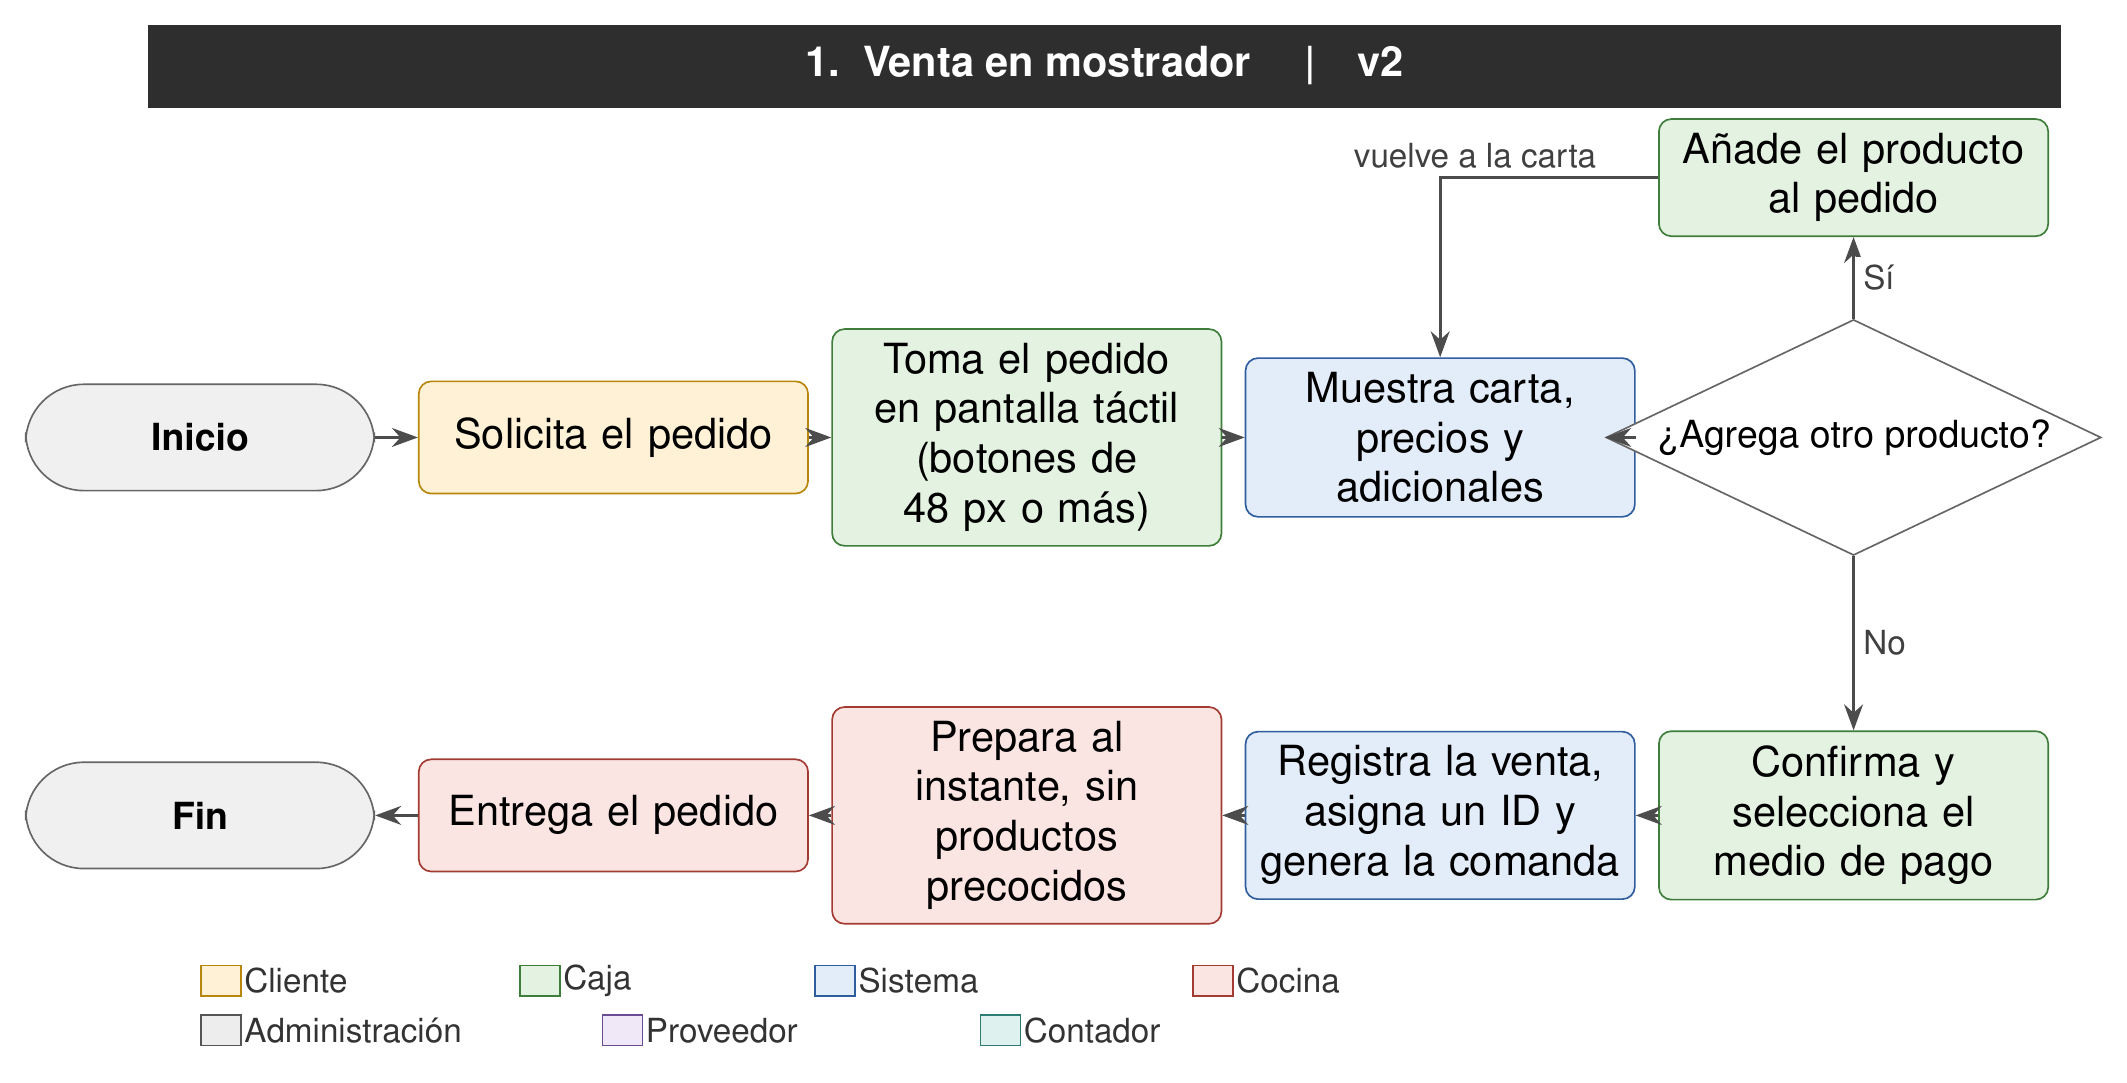
\includegraphics[width=\linewidth]{01-venta-mostrador.png}
  \caption{Diagrama 1: venta en mostrador. La caja toma el pedido en
  pantalla táctil; si el cliente agrega productos se vuelve a la carta y,
  al confirmar, el sistema registra la venta, asigna un identificador y
  genera la comanda que cocina prepara al instante.}
  \label{fig:venta-mostrador}
\end{figure}

\begin{figure}[H]
  \centering
  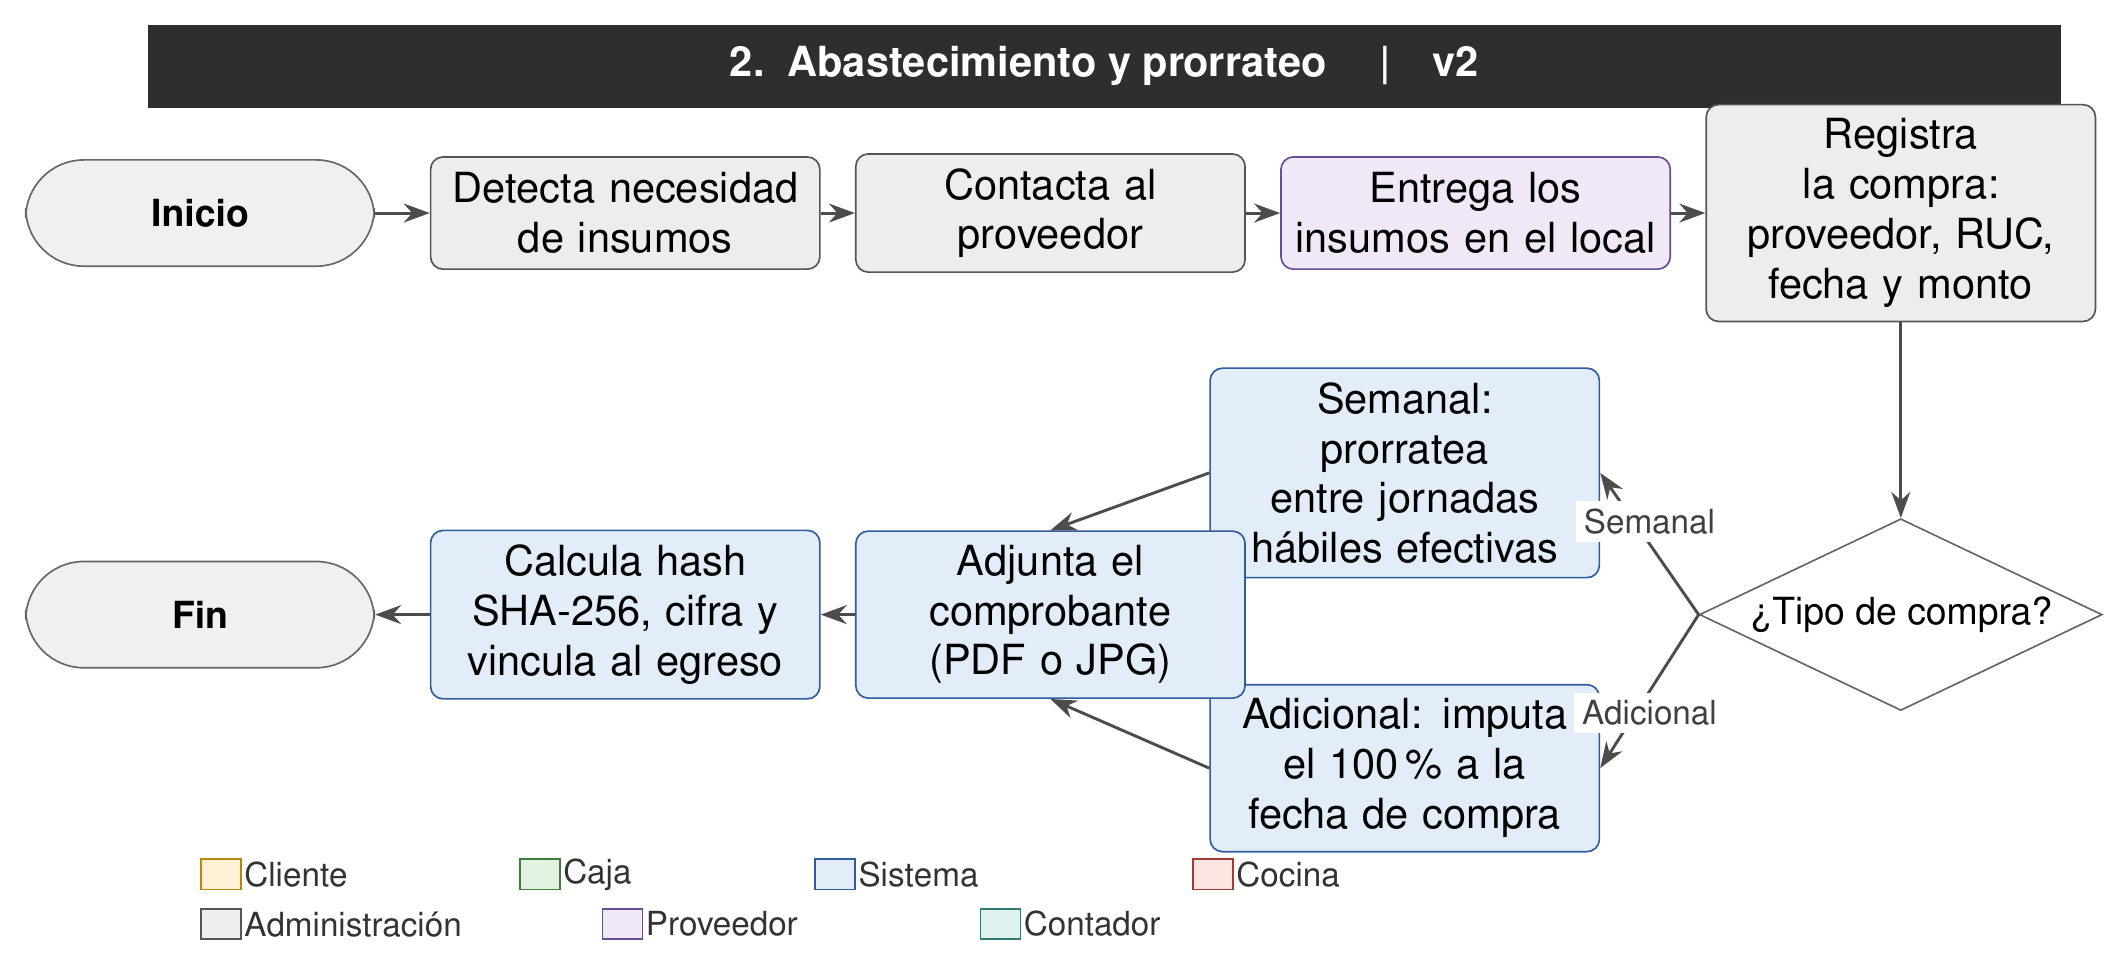
\includegraphics[width=\linewidth]{02-abastecimiento-prorrateo.png}
  \caption{Diagrama 2: abastecimiento y prorrateo. Tras registrar la compra
  se decide su tipo: la adicional se imputa al 100\,\% en la fecha de
  compra y la semanal se prorratea entre jornadas hábiles efectivas. En
  ambos casos se adjunta el comprobante, se calcula su hash SHA-256 —que
  verifica integridad, no cifra—, se cifra el archivo y se vincula al
  egreso.}
  \label{fig:abastecimiento}
\end{figure}

\begin{figure}[H]
  \centering
  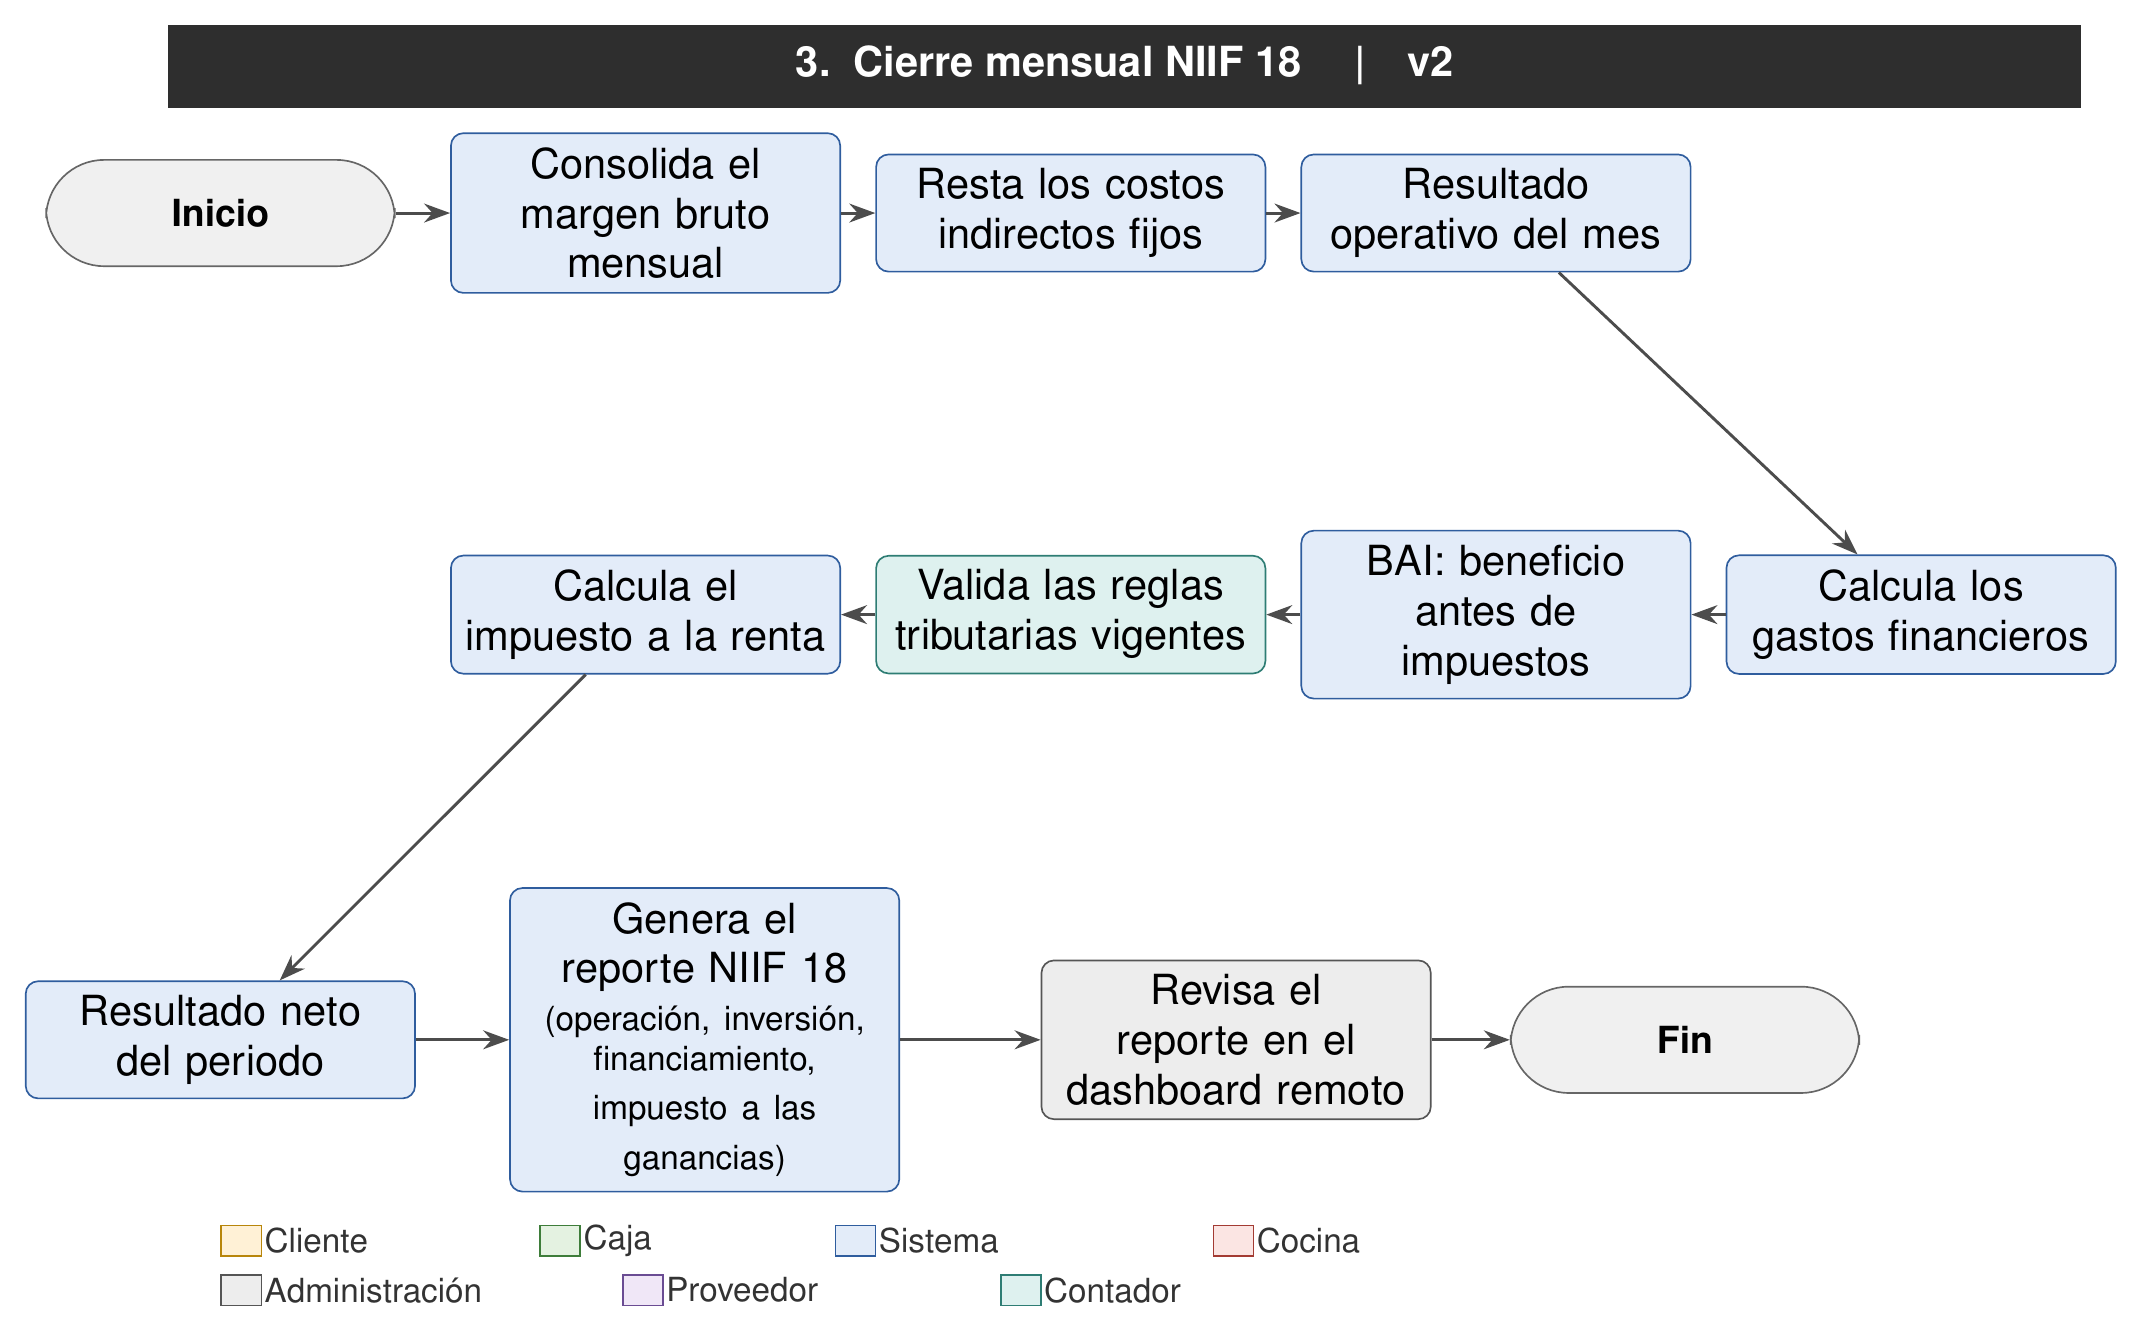
\includegraphics[width=\linewidth]{03-cierre-mensual-niif18.png}
  \caption{Diagrama 3: cierre mensual NIIF 18. Del margen bruto mensual se
  restan los costos indirectos fijos y se obtiene el resultado operativo;
  luego se deducen los gastos financieros para llegar al BAI, el contador
  valida las reglas tributarias, se calcula el impuesto a la renta y se
  llega al resultado neto, que alimenta el reporte NIIF 18.}
  \label{fig:cierre-mensual}
\end{figure}

\begin{figure}[H]
  \centering
  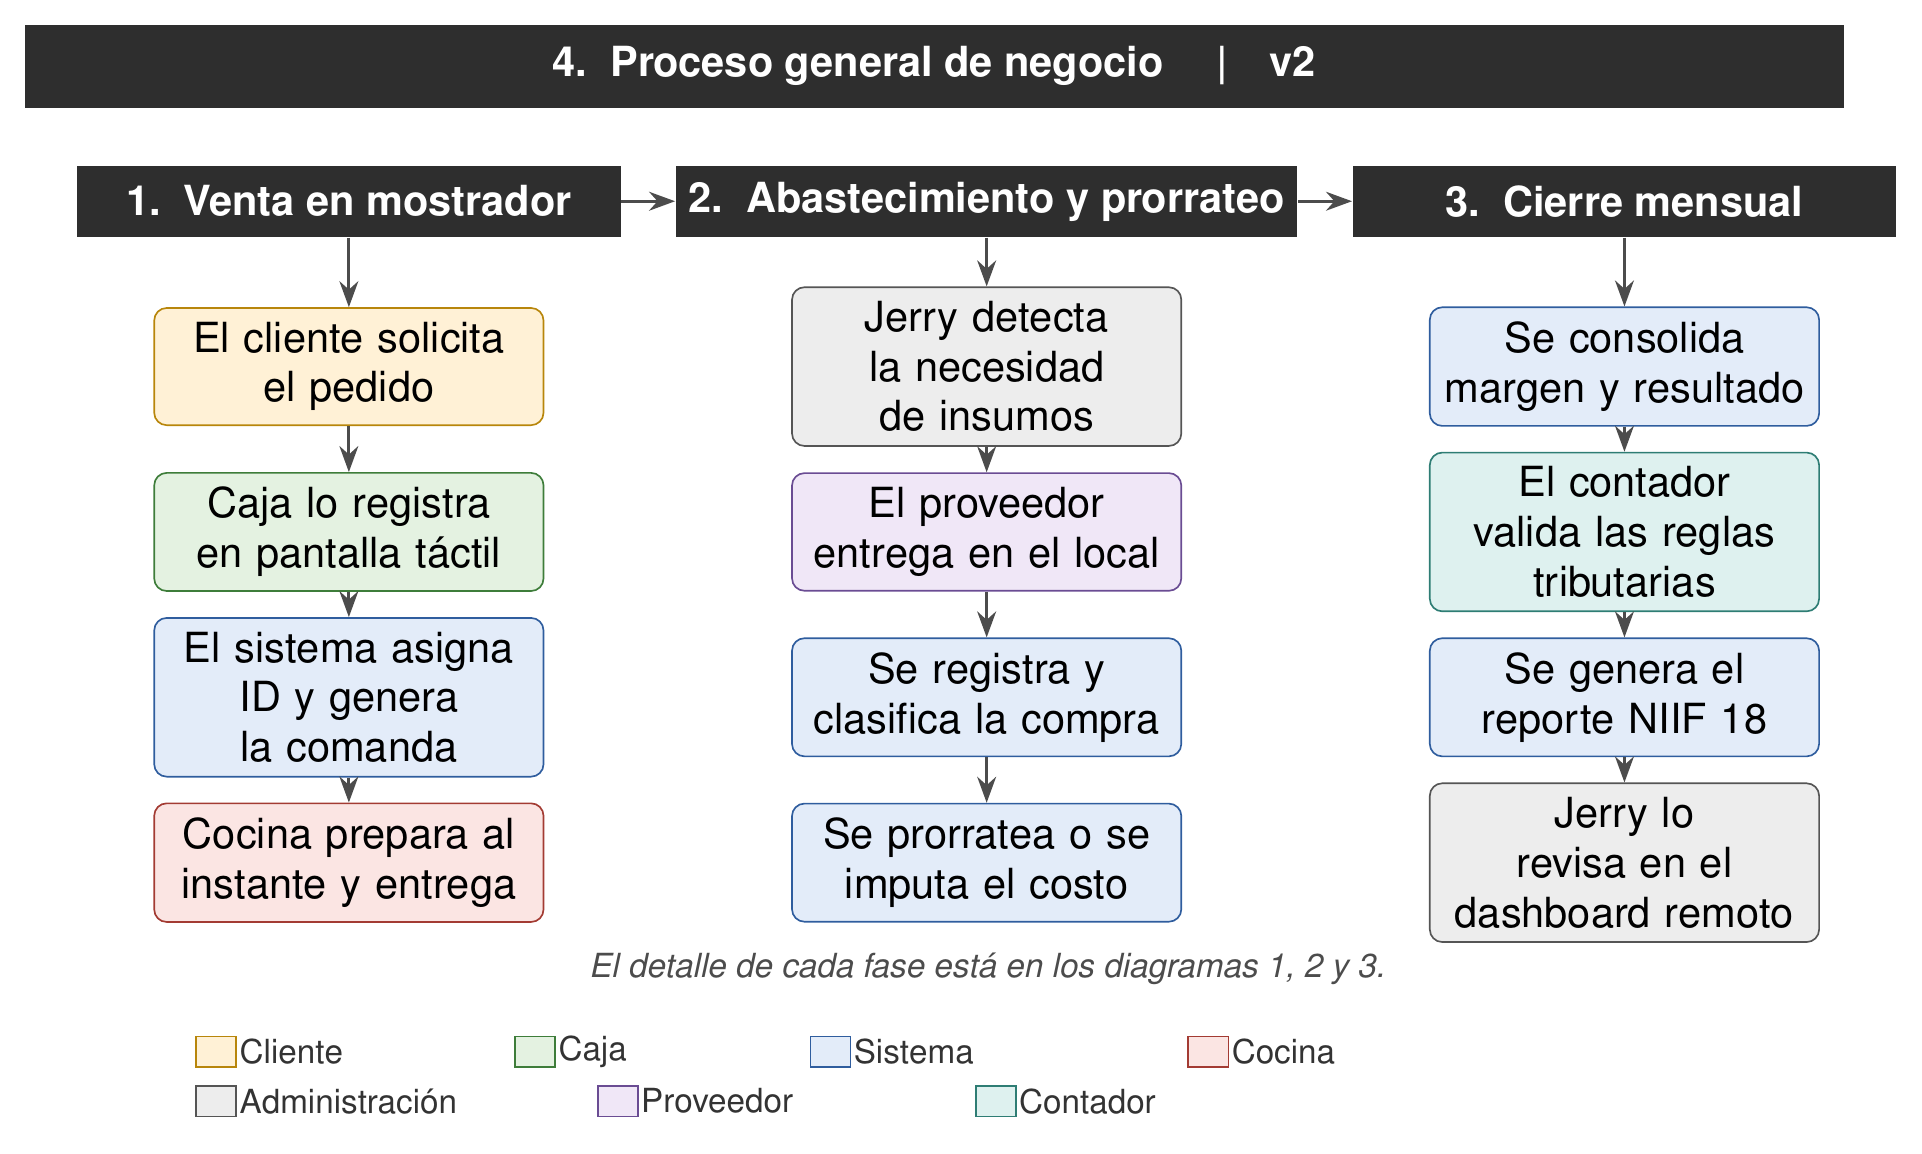
\includegraphics[width=\linewidth]{04-proceso-general.png}
  \caption{Diagrama general del proceso de negocio de RedPepper. Resume el
  negocio en tres fases encadenadas —venta en mostrador, abastecimiento con
  prorrateo y cierre mensual— y remite a los diagramas 1, 2 y 3 para el
  detalle de cada una.}
  \label{fig:proceso-general}
\end{figure}
